\newpage
\section{Projektbeschreibung}

Beschreibung des Projektes...\\

\begin{minipage}{\textwidth}
    \begin{center}
        Caption for image
        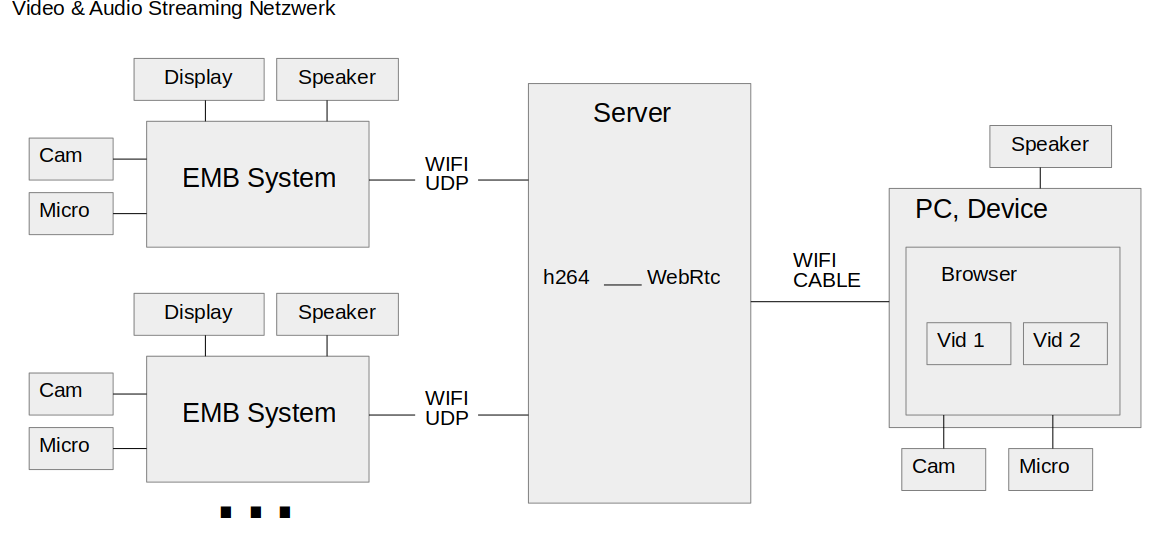
\includegraphics[scale=0.4]{img/schemaproj.png} 
    \end{center}
\end{minipage}

Beschreibung der Schritte zum erreichen des Projektes


\subsection{Streaming Basis Komponenten}
Streaming live convent over the internet requires much more extra care than just providing web page content since a downtime in the service can significantly affect the image of the company and cause it to lose content consumers and advertisers. There are several services on the internet that provide services to reliably stream audio and video content over the internet. However these paid services can be very expensive due to the importance of the availability of the service. Nevertheless, there is a cheaper alternative which is secure and reliable at the same time to set up an audio and/or video stream service on your own.

Any streaming service requires 3 components in order to work: a streaming server, a stream source and a client.

\textbf{Streaming server:}  This is the main component that passes (and sometimes re-encode) the audio and/or video content from each of the sources to the connected audience. There are several streaming servers both proprietary and open source that can be used. Among the open source alternatives, the most popular are Shoutcast and Icecast, both are easy to install and have proved to be very reliable and secure. To provide a single streaming point Shoutcast is the preferred option, however, to provide a more flexible service that allows multiple sources (different bitrates for example) Icecast might be more suitable. The advantage of Icecast over Shoutcast is that it introduces the concept of mountpoints which are independent streams mounted over the same server which distributes the resources efficiently among all the mountpoints. A Shoutcast example will be shown in this case.\\
\textbf{Stream Source:} A source provides the audio and/or video content to the streaming server. It usually provides capabilities to manage playlists and re-encode audio/video content. It does not need to be on the same physical server as the streaming server but it is recommended to be on a different server. A plugin for Winamp can be used as a source for a Shoutcast server which basically will send any content played on Winamp to a Shoutcast stream server. Liquidsoap is very powerful and programmable streaming source that allows generating a reliable streaming with fallback options. Liquidsoap can be used with either Icecast or Shoutcast. In addition, Liquidsoap provides a very strong a powerful API that allows generating different playlists, introducing jingles and defining fallback sources to produce a continuous streaming in case the main source becomes unavailable. Fallback is also available at server level in Icecast to provide an even more reliable streaming. The liquidsoap API also provides DSP (Digital Signal Processing) capabilities that allow programmatically mixing tracks, normalizing and controlling volume, and even introducing some effects. In this example, A simple Liquisoap script will be shown\\
\textbf{Client:} A client is referred to the software being used by the consumer to playback the stream.  This can vary greatly and depends on the preference of each user, but most of the current players (WMP, Quicktime, Winamp, iTunes, etc) will be able to playback audio streams in mp3 and other widely used formats. Some players provide plug-ins so streams can be played directly from the web browser. Other common formats in audio streams are aac+, asf, and ogg.




